\chapter{Design} 

In order to bridge the information gap regarding home energy systems, this study aims to provide households with knowledge of available technologies in the market. 
To address the potential issue of information overload, the study proposes a home energy system recommender to present households with a tailored selection of technologies that better fit their unique home situations, 
such as by learning the location of the house, in order to estimate the amount of sunlight it is likely to receive over the course of a year, to evaluate whether installing a \gls{pv} system would be a viable and effective way for the household.
The learning theory suggests that individuals learn new knowledge by connecting it with existing knowledge and experiences, as this helps to create a framework for understanding and retention of the new information.
Therefore, by focusing on personalised recommendations, the study hypothesises that households may be more receptive to learning about home energy technologies. 
Additionally, with the intention of nudging house owners towards making informed decisions. 

\section{Design concept}
The design concept of the home energy system recommender involves the utilisation of personalised recommendations based on the unique situations of households. 
By gaining a deep understanding of the household's energy demands and supply dynamics, the recommender can offer tailored recommendations to optimise energy efficiency and costs. 
Through this approach, the recommender not only provides guidance on these technologies but also educates the house owners on the potential benefits of transitioning to more sustainable energy sources. 
To ensure the effectiveness of the recommendations, clear and concise explanations are provided to enable users to make informed decisions.


\section{Input to the system}


\subsection{Household profiles}

The concept of household profile has been developed to gain insights into the energy demand and supply dynamics of households. 
To ensure the accuracy of this profile, various factors that may impact the household's energy consumption must be taken into consideration, as shown in Figure \ref{fig:profile}, including 
\emph{
    the external environment, 
    building materials, 
    energy consumption behaviors, 
    and the current home energy system. 
}
By creating such a profile, a comprehensive understanding of the household's situation can be attained, enabling the offering of more tailored and effective recommendations.
\begin{figure}[h]
    \centering
    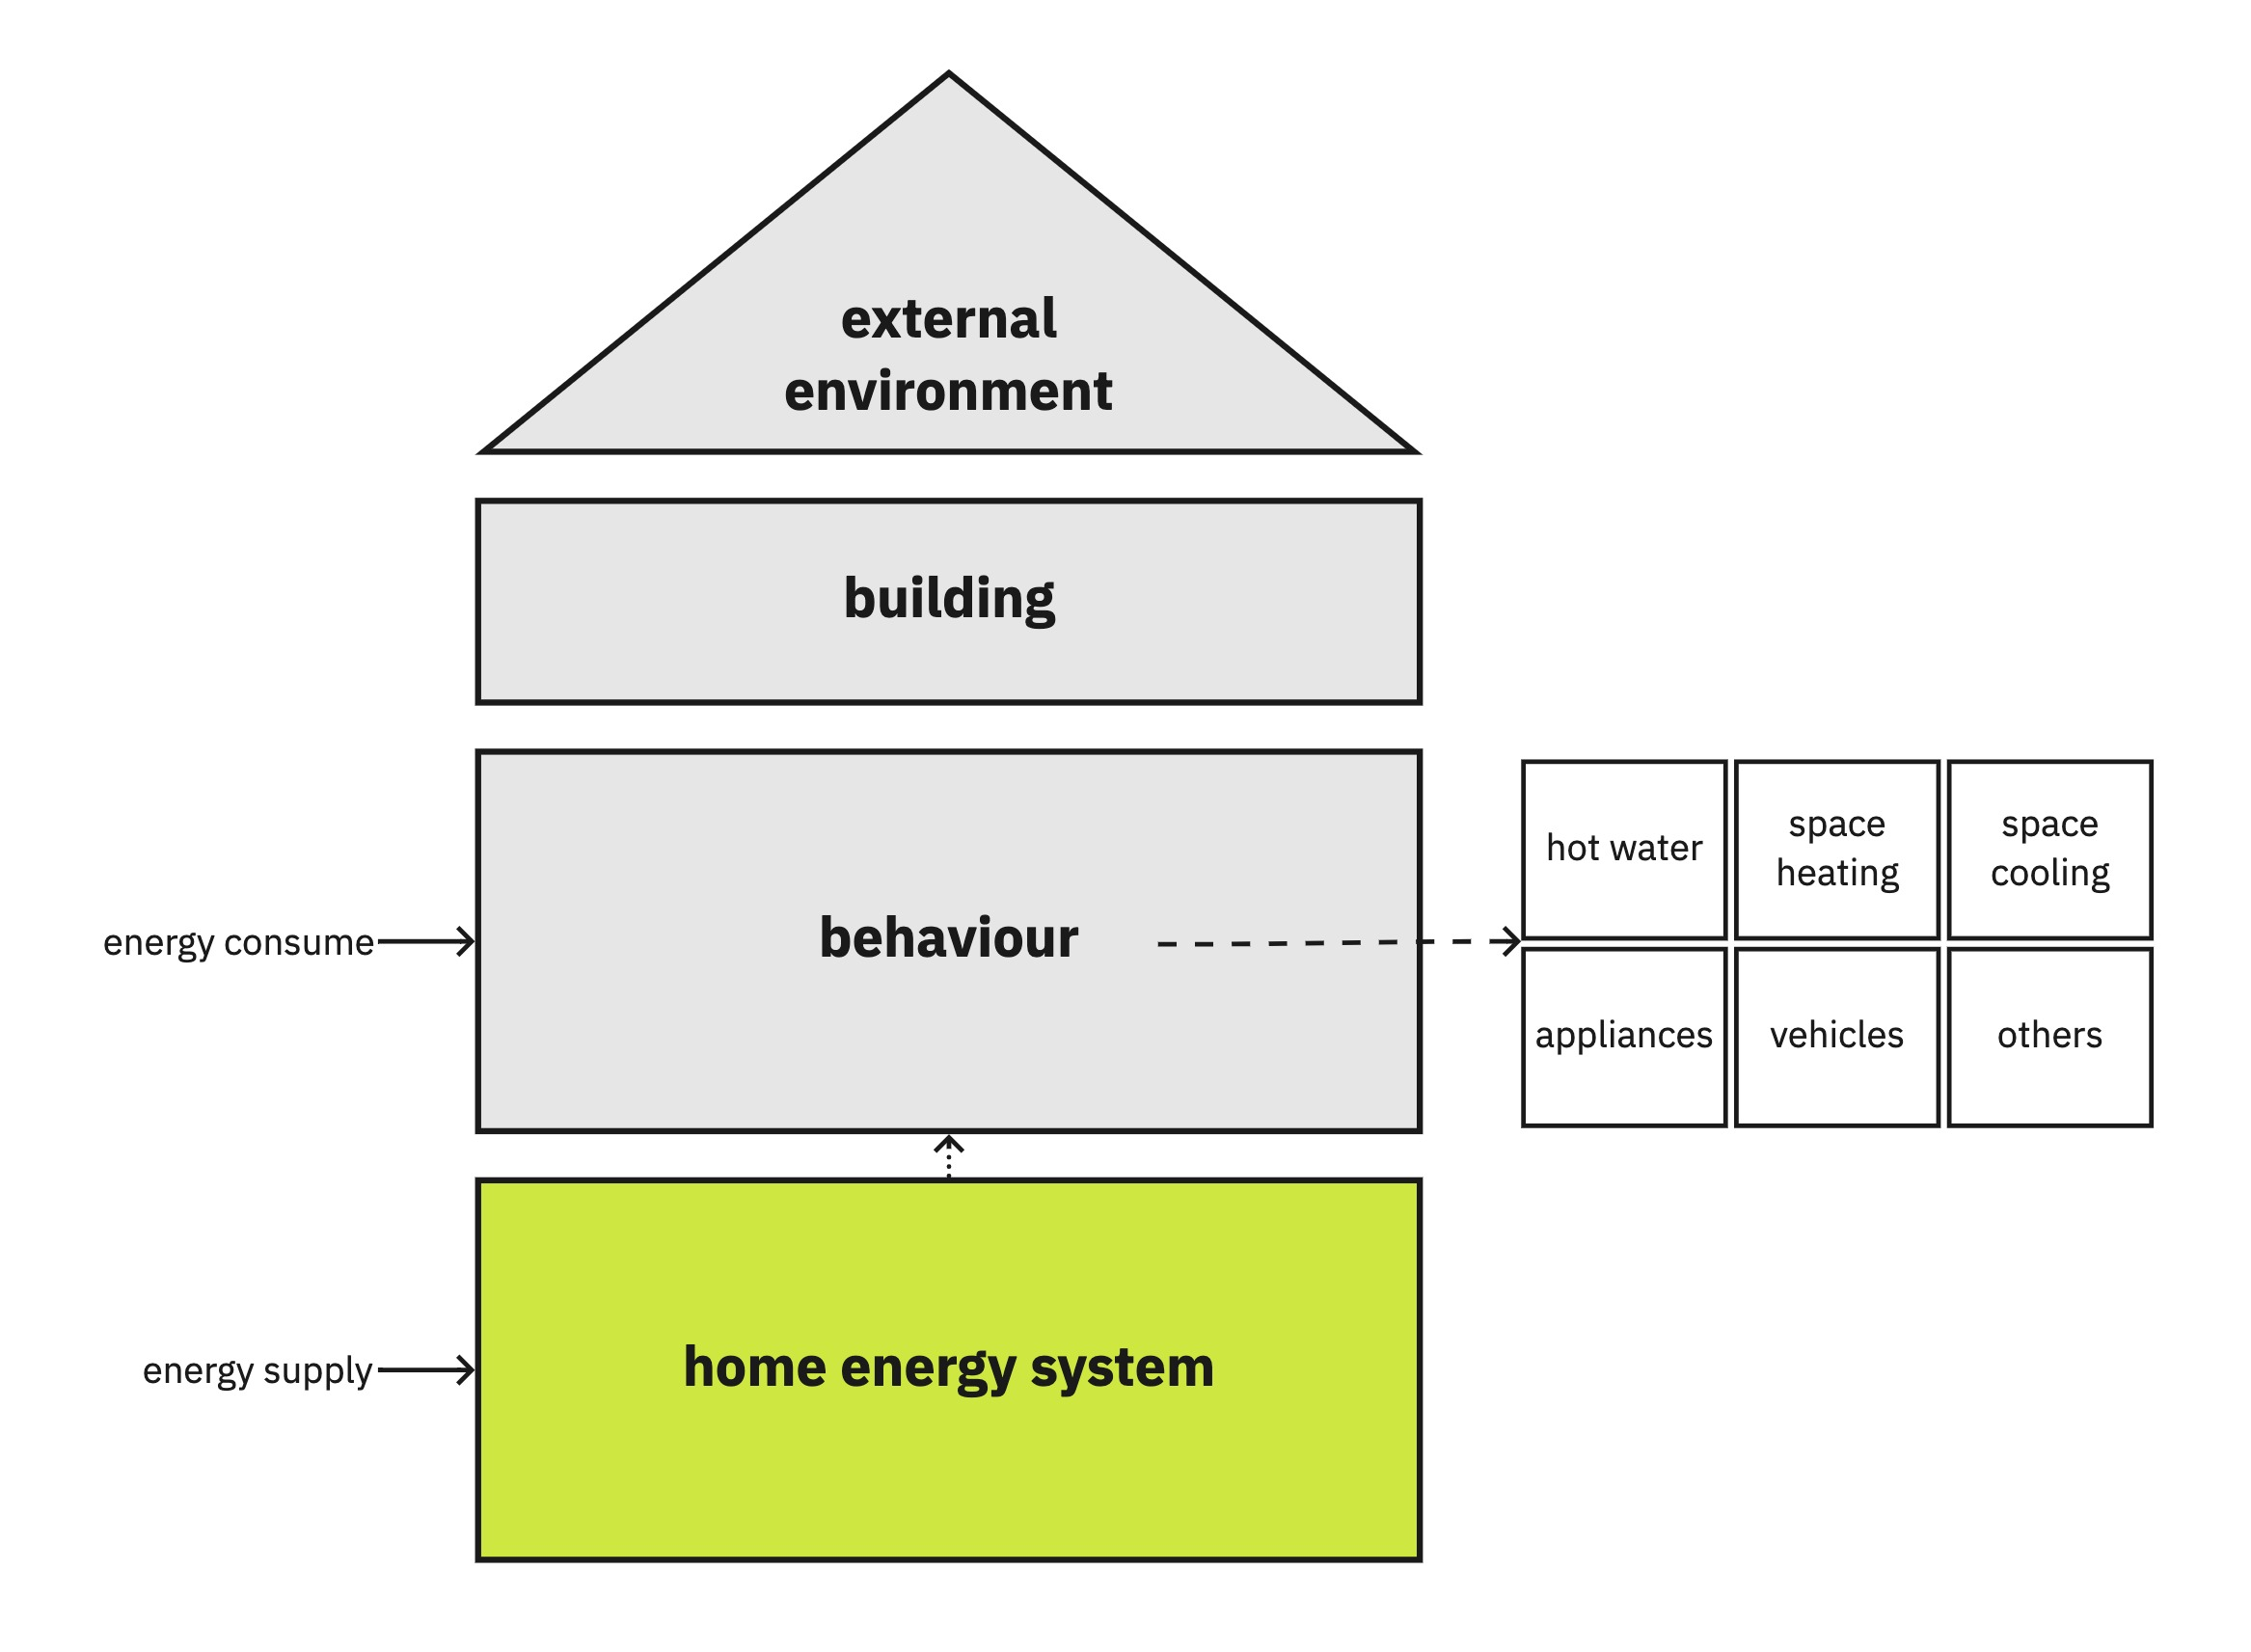
\includegraphics[width=\textwidth]{Images/household_profile.jpg}
    \caption{Household profile}
    \label{fig:profile}
  \end{figure}

\subsubsection{Input data by FLEX models}

In order to accurately anticipate household's energy costs,
the FLEX-Operation model takes a set of variables into account,
and they can be divided into following 15 categories: 
\emph{
    behaviour profile,
    battery,
    behaviour, 
    boiler,
    building,
    energy price,
    heating element, 
    hot water tank,
    \gls{pv},
    region,
    space cooling technology,
    space heating tank,
    vehicle,
    energy price,
    region weather. 
}
Furthermore, the specific data required by the FLEX-Operation model within each category can be found in Appendix \ref{appendix:inputdata}. 


\subsection{Decision trees for asking questions}

A total of 14 questions, see Table \ref{tab:questions}, were raised to collect all the relevant information necessary for the household profile analysis. 
In order to optimise the user experience, a decision tree approach was employed, allowing users to navigate through the questionnaire without the need to answer all the questions. 

\begin{center}
    \small
    \begin{longtable}{ | p{.15\textwidth} | p{.35\textwidth} | p{.35\textwidth} | }
        \hline
        Category & Question & Note \\
        \hline
        External environment & Where is the house located? & Understanding the location of the house can provide valuable insight into its environmental factors, such as the amount of sunlight it receives. \\
        \hline
        House condition & When was the house built? & Knowing the year a house was built can provide insight into its construction materials, such as the composition of the walls. \\
          & Has the house ever been renovated before? & Renovations can include upgrading insulation, replacing windows with energy-efficient ones, installing high-efficiency HVAC systems, sealing air leaks, etc. \\
          & What have been renovated in the house? &   \\
        \hline
        Energy use & How many people are living in the house? &   \\
          & How often does each adult work from home? &   \\
          & Is there any air conditioner in the house? &   \\
          & What type of heating energy is used in the house? &   \\
        \hline
        Home energy system  & Is there a photovoltaic (PV) system in the House? & A PV system is a system that uses solar panels to convert sunlight into electricity for use in a building. \\    
          & What is the size of the \gls{pv} system? &  The average size of a \gls{pv} system is 5 kilowatt-peak. \\
          & Is there a battery system in the house? & A home battery system is a device that stores energy produced by solar panels or other sources to be used later when needed. \\
          & What is the capacity of the battery? & The average capacity of a home battery system is around 7 kilowatt-hours. \\
          & Is there a smart energy management system in the house? &   \\
        \hline
    \caption{Survey questions}
    \label{tab:questions}
    \end{longtable}
\end{center}



\section{Output to the system}

\subsection{Recommendations}

An effective home energy system should prioritize minimizing energy waste, reducing dependence on non-renewable fossil fuels, and lowering overall energy costs. Our recommendations are aligned with these fundamental principles and aim to promote sustainable energy practices while also reducing household energy expenditures. 

The objectives of the recommendation system are multi-fold. 
Firstly, the system aims to support homeowners in making informed decisions regarding investments in home energy systems. 
Additionally, the system intends to encourage behavior change among homeowners by promoting the utilization of renewable energy sources. 
Finally, the recommendation system seeks to continuously refine and improve the accuracy of its predictive model, ensuring that the recommendations provided are up-to-date and effective. 
By providing users with tailored recommendations, the system aims to facilitate the adoption of energy technologies, ultimately leading to reduced energy demand and associated costs. 

As noted by Karen Palmer et al. \cite{informationgap}, financial considerations are of primary importance to homeowners when making decisions about energy investments. 
In line with this understanding, the recommendation system places a strong emphasis on providing transparent cost estimates for energy bills as well as recommended home energy system configurations. 
Additionally, the system seeks to encourage behavior change by providing information and education on climate change and renewable energy sources, aimed at increasing user awareness and understanding of the benefits of sustainable energy practices. 
To facilitate ongoing improvement and refinement of the recommendation system, a feedback survey button will be incorporated, allowing users to provide both short-term and long-term feedback on the system's performance and recommendations. 

\subsection{Explainability}

In order to provide more comprehensive and understandable recommendations, we have chosen to explain our recommendations from multiple perspectives beyond just cost estimates. 
Specifically, we have identified 4 key objectives, including \emph{trust, effectiveness, education, and debugging}, as key aspects to incorporate into our explanations. 
\emph{Trust}, we build trust with our users by using reliable data sources and providing transparent services. 
\emph{Effectiveness}, we strive to enhance the effectiveness of our service by offering recommendations that could actually benefit users economically. 
\emph{Education}, we seek to educate our users on the importance of environmental protection by sharing relevant knowledge and insights. 
\emph{De-bugging}, we value user feedback as an important tool for identifying and resolving any issues or bugs in our system, allowing us to continuously improve and refine our service.
The reasons for offering such explanations are to familiarise users with these technologies, establish accountability in the decision-making process, and encourage a shift towards environmentally conscious behaviour.
By incorporating these concepts into our explanations, we aim to provide recommendations that are transparent, trustworthy, understandable, and user-centred. 

Our recommendation system employs a three-level explainability framework to enhance user understanding of the recommended home energy system configurations. 
At the first level, the system provides an explanation in terms of the expected energy bill for the household. 
At the second level, the system offers a behavioural explanation of energy consumption patterns and the factors driving them. 
Finally, at the third level, the system aims to increase users' awareness and understanding of renewable energy and environmental protection.

Furthermore, the explanation is divided into three layers. 
At the first layer, users are provided with a comprehensive summary of their current energy consumption patterns. 
At the second layer, users are introduced to the various functionalities and benefits of the recommended energy technologies, including cost-saving potential and environmental impact. 
Finally, at the last layer, users are presented with simulated energy demand and supply data, allowing them to see the potential energy savings that could result from adopting the recommended configurations. 

Through the implementation of a comprehensive approach to explainability, our objective is to offer users an overview of energy technologies, enabling them to gain insight into their energy consumption patterns and to recognize the advantages of shifting towards more sustainable energy systems.


\subsection{Investments}

\begin{center}
    \begin{table}[h]
    \small
        \begin{tabular}{ | p{.30\textwidth} | p{.15\textwidth}  p{.15\textwidth}  p{.15\textwidth}  p{.15\textwidth} | }
            \hline
            Technology & \multicolumn{4}{ c | }{Cost (\euro{})} \\
             & Lowest & Highest & Installation & Maintenance \\
            \hline
            \gls{pv} system & \SI[per-mode=symbol,bracket-unit-denominator = false]{1957,68}{\per\kW}p & \SI[per-mode=symbol,bracket-unit-denominator = false]{2231,76}{\per\kW}p & included & 0 \\
            Battery system & \SI[per-mode=symbol,sticky-per,bracket-unit-denominator = false]{790,80}{\per\kWh}  & \SI[per-mode=symbol,sticky-per,bracket-unit-denominator = false]{2520,00}{\per\kWh} & included & 0 \\
            \gls{sems} & / & 1516,11 & 379,03 & 0 \\
            \gls{hp}& \SI[per-mode=symbol,bracket-unit-denominator = false]{432,15}{\per\kW} & \SI[per-mode=symbol,bracket-unit-denominator = false]{2370,31}{\per\kW} & included & 0 \\
            Hot water tank & 1 & 1 & 1 & 0 \\
            Space heating tank & 1 & 1 & 1 & 0 \\
            Air conditioner & 1 & 1 & 1 & 0 \\
            Basement renovation & \SI[per-mode=symbol]{132,12}{\per\metre\squared} & \SI[per-mode=symbol]{157,64}{\per\metre\squared} & included & 0 \\
            Roof renovation & \SI[per-mode=symbol]{40,95}{\per\metre\squared} & \SI[per-mode=symbol]{409,38}{\per\metre\squared} & included & 0 \\
            Wall renovation & \SI[per-mode=symbol]{67,57}{\per\metre\squared} & \SI[per-mode=symbol]{408,93}{\per\metre\squared} & included & 0 \\
            Window renovation & \SI[per-mode=symbol]{364,63}{\per\metre\squared} & \SI[per-mode=symbol]{958,92}{\per\metre\squared} & included & 0 \\
            \hline
        \end{tabular}
    \caption{Investment costs of different technologies}
    \label{tab:investments}
    \end{table}
\end{center}


\section{Interactions}

\subsection{Interfaces}

To facilitate user understanding of the recommended home energy system configurations and associated costs, our recommendation system will employ a visual and natural language explanation interface. 
Specifically, an interactive visualization tool will be implemented to enable users to explore and compare different energy system configurations in terms of energy consumption patterns and costs. 
Additionally, natural language explanations will be provided to further enhance user understanding and engagement with the recommended configurations. 


\subsection{Data visualisation}


